\documentclass{article}
\usepackage{graphicx} % Required for inserting images

\title{CSE305 N-Body Simulation Project Report}
\author{Daniela Cojocaru, Gabriel Faes, Aya Matmata}
\date{June 2025}

\begin{document}

\maketitle

\section{Introduction}
The N-body problem is a classic challenge in computational physics and computer science, involving the prediction of individual motions of a group of celestial objects interacting with each other gravitationally. Due to the quadratic growth in computational complexity as the number of bodies increases, efficient simulation of such systems is both a practical and theoretical concern. This report presents our implementation of an N-body simulation, focusing on both sequential and parallel approaches. We analyze the performance of our solution under varying numbers of bodies, simulation steps, and threads, and discuss the trade-offs and bottlenecks encountered. The results provide insight into the scalability of parallelization strategies for computationally intensive simulations.

\section{Approach}
Using the input data, the N-body simulation function updates an array (stored on the heap) which stores the position of every body on every time step. Every time step, knowing the current mass, position, and velocity of every body, the function updates every position and velocity using the time step length. Importantly, the function first updates velocities and then positions (this is an arbitrary decision, but may result in drastically different simulations compared to the reverse order).\\

To update the positions of every body, the function is split into two parts which run every time step. First, the “force calculation” portion of the function which, for every pair of bodies, calculates the x and y force on each of the two bodies and stores this in a “force” matrix (an array stored on the heap). Second, the “body calculation” portion of the function which, for every body, updates its velocity by summing the forces on the corresponding row of the force matrix, and then its position using that new velocity.\\

This algorithm works sequentially and already avoids calculating the force of each body twice. To make this parallel, each of the two parts of the function are individually parallelized. Each time step, the “force calculation” portion is split equally into the number of threads dictated and then rejoin before the “body calculation” portion is also split back into the number of threads and then rejoined again. While this creates a lot of threads every single time step, thread creation becomes comparatively cheap when the number of bodies starts nearing 1000. This immediately avoids using any mutexes and atomics, as any individual thread is never writing in the same place (the “force calculation” threads do read the position of bodies concurrently, but those values do not change before all threads rejoin).\\

The “body calculation” threads are simply given n/t bodies to update, where n is the number of total bodies and t is the number of threads available. The “force calculation” threads operate slightly differently, as calculating the forces for the first row of the matrix requires n-1 loops while calculating the forces of the second to last row requires a single calculation loop (since the matrix is symmetrical). Therefore, each thread is given approximately the same number of “calculation loops” to compute by the main thread, which ensures an even computational spread across all the threads.

\section{Testing machine}
Specs of the machine we ran the tests on:

Processor: Intel® Xeon (R) W-1290P\\
10 cores for a total of 20 logical processors\\
Lab Computer

\newpage
\section{Benchmarks}
\subsection{For varying body count}

\begin{figure}
        \centering
        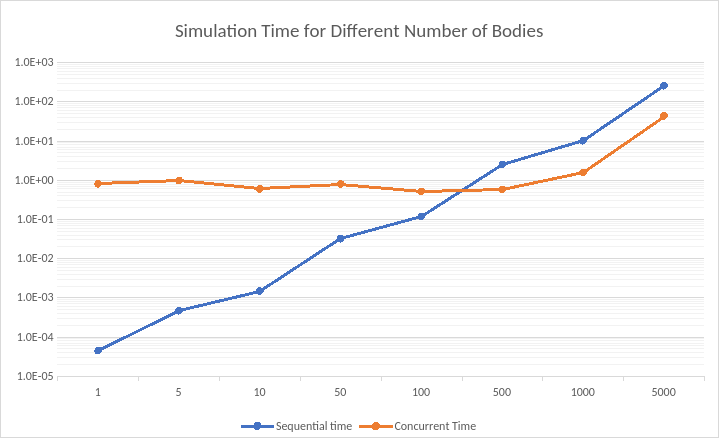
\includegraphics[width=1\linewidth]{graph.png}
        \caption{Enter Caption}
        \label{fig:enter-label}
\end{figure}
Computed for 1000 steps with 16 threads



\begin{table}[h]  
  \centering
  \begin{tabular}{|c|c|c|c|}
    \hline
    Bodies & Sequential time & Concurrent Time & Speedup \\ \hline
    1 & $4.50\times 10^{-5}$ & 0.812 & Slowdown! \\ \hline
    5 & $4.70\times 10^{-4}$ & 0.977 & Slowdown! \\ \hline
    10 & $1.49\times 10^{-3}$ & 0.602 & Slowdown! \\ \hline
    50 & 0.032 & 0.800 & Slowdown! \\ \hline
    100 & 0.119 & 0.517 & Slowdown! \\ \hline
    500 & 2.525 & 0.580 & 4.35 \\ \hline
    1000 & 10.227 & 1.585 & 6.45 \\ \hline
    5000 & 257.599 & 43.380 & 5.94 \\ \hline
  \end{tabular}
  \caption{Performance Table}
  \label{tab:performance_table}
\end{table}


Times are listed in seconds
$O(n^2)	$Still $O(n^2)$ sadly, starting at around 1000 bodies				
						
The slowdown for <500 bodies is created because of excessive thread creation (15 threads, 16-1, are created twice every time step, no matter if they are performing calculations or not, which is 30000 threads)					

\subsection{For varying step count}
Performed with 1000 bodies and 16 threads
\begin{table}[h]
  \centering
  \begin{tabular}{|c|c|c|c|}
    \hline
    Steps & Sequential Time & Concurrent Time & Speedup \\ \hline
    10 & 0.122 & 0.021 & 5.86 \\ \hline
    100 & 1.062 & 0.149 & 7.13 \\ \hline
    1000 & 10.316 & 1.492 & 6.91 \\ \hline
    10000 & 99.432 & 14.945 & 6.65 \\ \hline
    & $O(n)$ & $O(n)$ & \\ \hline
  \end{tabular}
  \caption{Performance comparison of sequential and concurrent executions as a function of step count}
  \label{tab:performance_comparison}
\end{table}

		
Expectedly linear				

\subsection{For varying thread count}
Computed for 1000 steps and 1000 bodies.
Sequential Time: 10.3

\begin{table}[h]
  \centering
  \begin{tabular}{|c|c|}
    \hline
    Threads & Concurrent Time \\ \hline
    2  & 16.584 \\ \hline
    4  & 4.103 \\ \hline
    8  & 1.900 \\ \hline
    16 & 1.788 \\ \hline
    20 & 1.599 \\ \hline
    24 & 2.129 \\ \hline
    32 & 2.122 \\ \hline
    64 & 2.633 \\ \hline
    128 & 6.227 \\ \hline
  \end{tabular}
  \caption{Concurrent Times for Different Thread Counts}
  \label{tab:concurrent_times}
\end{table}
	

Speed up until 20 threads, which makes sense given the 20 logical threads the computer has.		

\section{Work distribution}
The work was distributed among the team members as follows: Daniela was responsible for implementing the main thread logic, Gabriel focused on developing the simulation threads, and Aya worked on the graphical representation of the simulation.

\section{Conclusion}
In conclusion, our implementation and analysis of the N-body simulation demonstrate both the challenges and opportunities inherent in parallelizing computationally intensive algorithms. While parallelization offers significant speedup for large numbers of bodies and steps, it introduces overhead that can outweigh its benefits for smaller problem sizes. Our results show that careful consideration of thread management and workload distribution is essential to achieve optimal performance, especially as the number of available logical processors increases. Future work could explore more advanced parallelization techniques, such as thread pooling or GPU acceleration, to further improve scalability and efficiency. Overall, this project provided valuable insights into the practical aspects of high-performance computing and parallel programming.

\end{document}
